\chapter{Resultados}

Três testes com diferentes temperaturas de referência foram realizados para que fosse possível a análise da eficiência do regulador. Nos três testes, a temperatura ambiente encontrava-se por volta de 27$^{\circ}$C. Os dados de temperatura foram adquiridos utilizando-se o próprio sensor LM35.

    O primeiro teste foi realizado com a referência (temperatura desejada da água) para 34$^{\circ}$C. A figura 5.1 mostra o gráfico da temperatura da água em função do tempo.
    
\begin{figure}[H]

\center

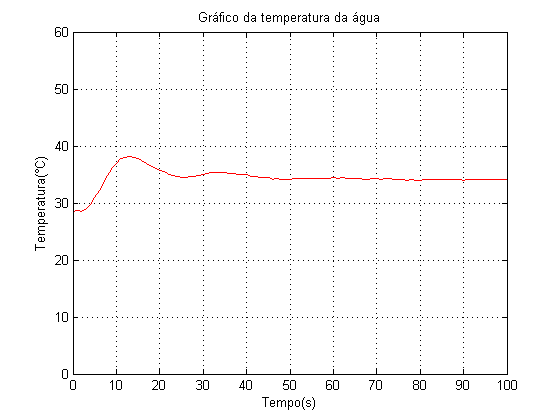
\includegraphics[width=10cm]{imagens/grafico_34graus.png}

\label{Temperatura da água para referência em 34 graus Celsius}

\caption{Temperatura da água para referência em 34 graus Celsius}
\end{figure}
    
\noindent É possível notar uma pequena variação na temperatura após o sistema atingir o regime permanente (cerca de 40 segundos). Essa variação, apesar de não influenciar de forma relevante na variação da temperatura, provavelmente se dá devido ao ruído do sensor LM35. 

    Mesmo com a presença de ruídos no sensor de temperatura, o regulador teve uma eficiência satisfatória, com baixíssimas variações em relação a temperatura desejada, que dificilmente seriam notadas na pele de uma pessoa.

O segundo teste realizado foi para a temperatura desejada de 37$^{\circ}$C. A figura 5.2 mostra o gráfico para o teste realizado.
\begin{figure}[H]
\center

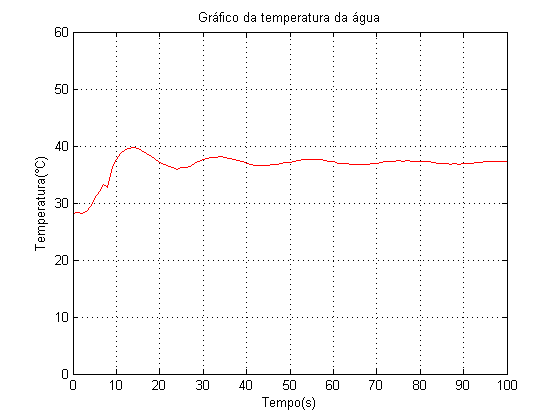
\includegraphics[width=10cm]{imagens/grafico_37graus.png}

\label{Temperatura da água para referência em 37 graus Celsius}

\caption{Temperatura da água para referência em 37 graus Celsius}
\end{figure}

\noindent Neste caso pode-se perceber que o ruído no sensor teve uma influência maior, pois após o tempo de regime permanente as variações foram um pouco maiores que as analisadas no primeiro teste, porém, como o primeiro teste, essas variações seriam dificilmente notadas em um banho.

O terceiro e último teste foi realizado com a temperatura desejada de 40$^{\circ}$C. A figura 5.3 mostra o gráfico para o último teste.
\begin{figure}[H]
\center

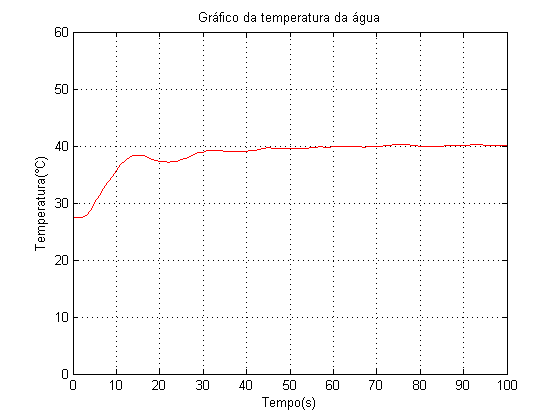
\includegraphics[width=10cm]{imagens/grafico_40graus.png}

\label{Temperatura da água para referência em 40 graus Celsius}

\caption{Temperatura da água para referência em 40 graus Celsius}
\end{figure}

\noindent O comportamento deste teste foi bastante semelhante ao do primeiro. As variações de temperatura após a estabilização foram baixíssimas, em torno de 0,2$^{\circ}$C à 0,3$^{\circ}$C.

Com base nos gráficos apresentados para os testes, pode-se notar que o regulador de temperaturas funciona de forma satisfatória com erros que variam em torno de  0,2$^{\circ}$C à 0,3$^{\circ}$C, valores que a pele humana dificilmente irá sentir em um banho. O tempo de ajuste de temperatura da água do banho foi reduzido de dois minutos (tempo médio para ajuste da temperatura ideal de um chuveiro convencional) para cerca de 40 segundos.